\section{Challenges}

While the performance improvement demonstrated on the code in Listing 1 is impressive, it is perhaps not representative of most Java code.  Java conventions encourage the use of indirection when accessing class fields using non-static {\em get} and {\em set} methods, as well as liberal use of exceptions.  Unlike C compilers, which assume a ``closed world'' and often inline simple functions into the body of calling methods to improve performance, the Java compiler must assume an ``open world'' in which a class may be used in a new context, so inlining of non-final methods is unsafe.

Previous approaches to veritesting exit static code regions when indirect calls to functions or non-local jumps are made.  In this section, we explore how the structure of Java programs reducees the performance of a n\"aive veritesting approach.

%Talk about how veritesting is different when done on Java bytecode
%
%The transition points at the Java bytecode level are return, exceptions (done using athrow), virtual function invocations (invokevirtual, invokeinterface), native calls (also done using invokevirtual), reflection and dynamic class loading (also done using invokevirtual).
%
%Present results from Soot-based static analysis
%
%Talk about how veritesting gets harder to do when considering multi-threaded Java bytecode.
\subsection{Exit Points}
\label{sec:exit_points}

\mike{Should we re-run this analysis with WALA for consistency's sake?}
%While the performance improvement shown in Figure~\ref{fig:v_ex_plot} with statically unrolling the three-way branches is clear, we need to automate this process.
%
Integrating veritesting with SPF requires that we can represent a region of a Java program as a disjunctive formula with multiple exit points.  Each exit point describes a possible distinct continuation of the current path after the static code region completes execution.  Avgerinos et al.~\cite{veritesting} defined exit points as unresolved jumps, function boundaries, and system calls.
%
These exit points are nodes in a control-flow graph which represent non-local control flow, and therefore, need to be explored using plain dynamic symbolic execution.
%
In the context of Java bytecode, we find such non-local control flow in five ways listed as follows: (1) return statements, (2) exceptions, (3) virtual function invocations~(\textit{invokevirtual}, \textit{invokeinterface}), (4) reflection, (5) native calls.
%
\iffalse
\mike{These explanations are obvious and can be dispensed with if we need space}
Return statements form the function boundary, and are obvious candidates to be considered as exit points.
%
Exceptions are used to catch unexpected behavior, and often help design of cleaner code, and allow developers to capture useful information when such errors occur.
%
Virtual function invocations occur due to runtime polymorphism supported by Java.
%
The runtime environment binds the method call to its body by using the type of the object making the call.
%
Using reflection requires loading a class at runtime, identifying a method within the class, and calling it.
%
It is primarily used for extensibility purposes, achieving separate compilation, and generating a class at runtime.
\fi
%
%An approach such as Avgerinos et al.~\cite{veritesting} would force
%static code regions when any of these five constructs are encountered.

%Such regions must correctly preserve the semantics of symbolic execution for all possible Java constructs.
%
The primary benefit of implementing veritesting comes from its conversion of branches into disjunctions in a multi-path region.
%
But this benefit exists only when the number of different exit points from the disjunctive formula is less than the number of execution paths through the region in the first place.
%
For example, all execution paths in the first three-way branch in
Listing~\ref{lst:v_ex} joined together on line 7, causing the three-way branch to have a single exit point.
%
Therefore, it is crucial for us to study the number of exit points for each of our statically-analyzed regions vs. the number of branches within the region.
%
%
%Native calls are used to execute code outside of the Java Runtime Environment.
%
%Incorporating these into our static analysis would require handling virtual function invocations as well as static analysis of binary code.

These five types of exit points create the kind of non-local control flow which formed the frontier of the visible control-flow graph created as a result of \textit{CFGReduce} step by Avgerinos et al.
%
However, many of these exit points are used pervasively by Java developers.
%
For example, the Visitor design pattern is used extensively by the ASM framework~\cite{asm}, Soot~\cite{soot} and makes use of Java\rq s dynamic dispatch mechanism.
%
Running into exit points too often causes our statically-analyzed regions to be small and our performance gain from having fewer branches to be lost.

We investigated the occurrence of these exit points by creating a Soot-based static analysis of six large open-source projects written in Java.
%
Software faults from these six projects are maintained in the Defects4J~\cite{defects4j} repository.
%
We used Soot to create a control-flow graph for every method body in every class file in these six projects.
%
For each control-flow graph, we used nodes corresponding to conditional jump bytecodes as a starting point of our analysis.
%
We measured the number of instructions encountered when traversing down each side of the branch until we get to the immediate post dominator~\cite{dragon-book} of our starting point.
%
If there were no exit points encountered on any side of the branch, we considered this region as a pure multi-path region and calculated its size in bytecode instructions.
%
Finally, we allowed up to five nested branches and calculated the number of bytecode instructions from the earliest, as well as, the latest starting point in our control-flow graph traversal to an exit point.

As an example, we modify the three-way branch in Listing~\ref{lst:v_ex} by adding a {\tt else return;} to get the snippet shown in Listing~\ref{lst:v_ex_modified}.
%
\lstinputlisting[caption={Listing~\ref{lst:v_ex} modified to have a return statement in the three-way branch},
label={lst:v_ex_modified}, language=Java]{code_samples/VeritestingPerf_modified.java}
%
This results in bytecode that produces the control-flow graph shown in Figure~\ref{fig:v_ex_cfg}.
%
Nodes are numbered 1 through 6 with node (1) being the starting point and node (6) being the immediate post-dominator of node (1).
%
Nodes contain bytecode instructions along with instruction offsets.
%
The added \textit{return} statement creates an exit point, which causes the three-way branch in Listing~\ref{lst:v_ex_modified} to contain two exit points.
%
Counting the number of instructions after the {\tt ifge} instruction in node (1) through node (2) to node (6) gives us two instructions.
%
The same count going through nodes (3) and (4) to (6) gives us 6 instructions, and through nodes (3) to (5) gives us 4 instructions.
%
The presence of the \textit{return} statement in node (5) prevents this region from being a pure multi-path region.
%
\begin{figure}[]
\caption{Control-flow graph with {\tt else return;} added as line 7 of Listing~\ref{lst:v_ex}}
\label{fig:v_ex_cfg}
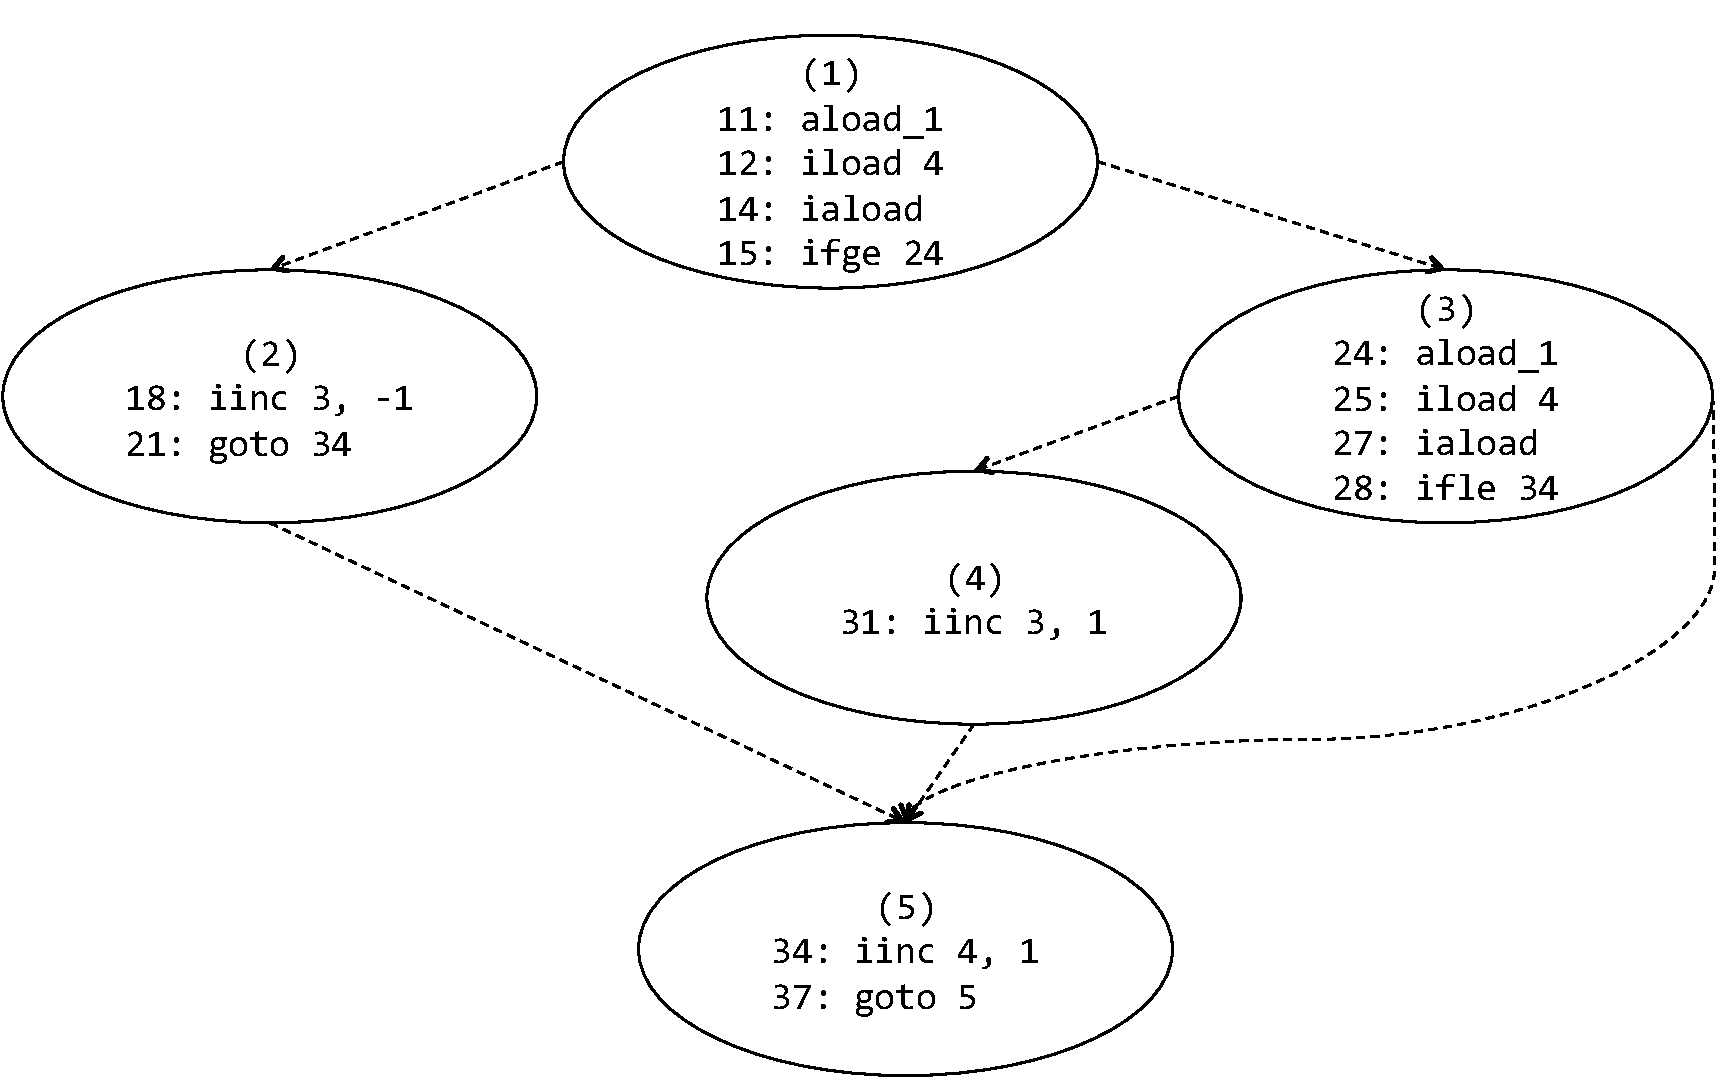
\includegraphics[width=\columnwidth]{figures/v_ex_cfg}
\end{figure}

%
We report our results from a Soot-based static analysis in Tables~\ref{t:r_s} and~\ref{t:r_c}.
%
\begin{table}[]
\centering
\begin{tabular}{|l|l|l|l|l|l|}
\hline
        & \#classes & \begin{tabular}[c]{@{}l@{}}if-\\ return\end{tabular} & \begin{tabular}[c]{@{}l@{}}if-\\ invokevirtual\end{tabular} & \begin{tabular}[c]{@{}l@{}}if-\\ throw\end{tabular} & \begin{tabular}[c]{@{}l@{}}region \\ size\end{tabular} \\ \hline
chart   & 679       & 8.44                                                 & 27.47                                                       & 4.33                                                & 13.59                                                  \\ \hline
closure & 1339      & 7.35                                                 & 22.1                                                        & 9.5                                                 & 11.66                                                  \\ \hline
lang    & 170       & 6.70                                                 & 11.64                                                       & 7.09                                                & 9.60                                                   \\ \hline
math    & 1104      & 18.27                                                & 56.61                                                       & 9.56                                                & 27.06                                                  \\ \hline
mockito & 382       & 6.02                                                 & 12.51                                                       & 8.05                                                & 13.57                                                  \\ \hline
time    & 209       & 7.79                                                 & 13.10                                                       & 7.08                                                & 8.10                                                   \\ \hline
\end{tabular}
\caption{Soot-based analysis for number of bytecode instructions between starting and exit points}
\vspace{-0.3in}
\label{t:r_s}
\end{table}
%
%\vspace{-0.7in}
%
\begin{table}[]
\centering
\begin{tabular}{|l|l|l|l|l|}
\hline
        & \begin{tabular}[c]{@{}l@{}}if-\\ return\end{tabular} & \begin{tabular}[c]{@{}l@{}}if-\\ invokevirtual\end{tabular} & \begin{tabular}[c]{@{}l@{}}if-\\ throw\end{tabular} & \begin{tabular}[c]{@{}l@{}}region\\ count\end{tabular} \\ \hline
chart   & 1712                                                 & 7760                                                        & 521                                                 & 6627                                                   \\ \hline
closure & 3853                                                 & 7466                                                        & 138                                                 & 9258                                                   \\ \hline
lang    & 3602                                                 & 1589                                                        & 539                                                 & 2065                                                   \\ \hline
math    & 2219                                                 & 5582                                                        & 662                                                 & 15375                                                  \\ \hline
mockito & 372                                                  & 572                                                         & 15                                                  & 574                                                    \\ \hline
time    & 1202                                                 & 984                                                         & 204                                                 & 1421                                                   \\ \hline
\end{tabular}
\caption{Number of occurences in Soot-based static analysis}
\vspace{-0.2in}
\label{t:r_c}
\end{table}
%
Table~\ref{t:r_s} shows the average size and Table~\ref{t:r_c} shows the number of times each such count was reported.
%\mike{We need to explain these tables better: can we take a small code fragment (say, that of Listing 1) and explain it according to these numbers, or create a very tiny code fragment that demonstrates them?}
%
The \textit{if-return}, \textit{if-invokevirtual}, \textit{if-throw} columns in Table~\ref{t:r_s} report the average number of instructions observed between any \textit{if} opcode-containing bytecode instruction and a \textit{return}, \textit{invokevirtual} or \textit{invokeinterface}, \textit{throw} opcode-containing bytecode instruction.
%
These same columns in Table~\ref{t:r_c} report the number of times we observed an occurence of one of \textit{return}, \textit{invokevirtual}, \textit{invokeinterface}, \textit{throw} opcode-containing bytecode instructions before reaching the immediate post-dominator of the starting \textit{if} node on any side of the branch.
%
Tables~\ref{t:r_s} and~\ref{t:r_c} show that while we discover thousands of regions which do not contain any exit points, these regions are small.
%
They also show that early \textit{return} instructions are another often used construct in Java.
%
We believe that creating multi-path regions for these no-exit-point cases alone would provide a significant performance boost to SPF.
%
Table~\ref{t:r_c} shows \textit{invokevirtual} or \textit{invokeinterface} instructions are encountered far more often than \textit{return} or \textit{throw} instructions.
%
This can be explained by the pervasive use of runtime polymorphism and exception handling by Java developers.
%
Instead of using \textit{invokevirtual} and \textit{invokeinterface}
instructions as exit points, if we can continue our predicate
construction for multi-path regions beyond them, we would almost double
the number of multi-path regions.
%

\iffalse
\subsection{Engineering Challenges}
Research challenges such as static analysis of exit points and veritesting in a multi-threaded context need to be solved for integrating veritesting with any bytecode-level symbolic execution engine.
%
Symbolic PathFinder is a popular Java bytecode-level symbolic execution tool.
%
It has been used to find bugs in flight software~\cite{pasareanu2008}, to test large web applications~\cite{fujitsu}, and for testing Android apps~\cite{android_spf}.
%
%It has also been extended for parallel symbolic execution~\cite{parallel}, and for load testing~\cite{load_testing_spf}.
%Talk about the engineering challenges we face when implementing veritesting with Symbolic PathFinder
%
Given the large and diverse set of applications that stand to benefit from integrating veritesting into SPF, we discuss here the engineering challenges expected with such an integration.
\fi

\subsection{Shared Expressions}
%Sharing implementation needs to be fixed. Show this using the TestSharing example
Veritesting causes regions of code to be executed using static symbolic execution.
%
Symbolic formulas representing the static symbolic execution are then gathered at the exit points of the region and added to the path expression and symbolic store of dynamic symbolic execution.
%
This causes large disjunctive formulas to be substituted and reused multiple times, necessitating the use of techniques like hash consing~\cite{hashconsing}, or its variants such as maximally-shared graphs~\cite{babic}, or using expression caching~\cite{green}.
%
To evaluate reuse of structurally equivalent expressions in SPF, consider the code shown in Listing~\ref{lst:sharing}.
%
\lstinputlisting[caption={An example with an increasing formula size with every loop iteration},
label={lst:sharing}]{code_samples/TestSharing.java}
%
The function \textit{testSharing} adds the value of \textit{x} to itself in every loop iteration on line 3 of Listing~\ref{lst:sharing}.
%
The number of loop iterations is controlled by a user-supplied value for \textit{bound}.
%
On line 4, the code branches on the value of the value of \textit{x}.
%
We symbolically executed the \textit{testSharing} method with \textit{x} set to be symbolic and \textit{bound} set to be a concrete value.
%
We set the minimum and maximum symbolic integer values to be -100 and 100 respectively.
%
We increased the value of \textit{bound} from 1 to 30 and recorded the time taken for complete path coverage.
%
Figure~\ref{fig:sharing} shows the trend seen in running time and memory
usage for increasing values of \textit{bound}.
%
Figure~\ref{fig:sharing_time} shows that the running time remains constant until the value for \textit{bound} is 18, and then starts to rise exponentially.
%
%We also recorded the maximum memory usage reported by SPF for increasing values of \textit{bound}, and present our observation in Figure~\ref{fig:sharing_mem}.
%
\begin{figure}%
    \centering
    \subfloat[Time required for covering paths in Listing~\ref{lst:sharing}]{{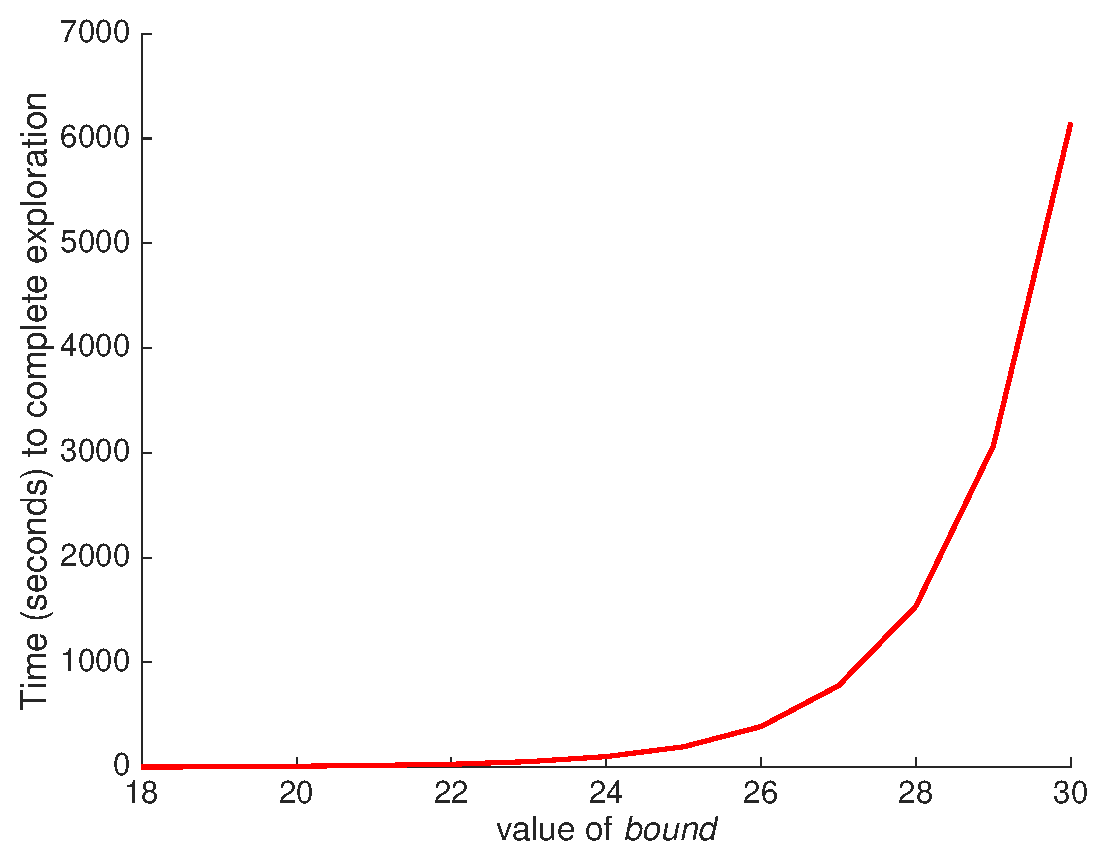
\includegraphics[width=0.4\columnwidth]{figures/sharing_time} }\label{fig:sharing_time}}%
    \qquad
    \subfloat[Maximum memory usage of SPF for covering paths in Listing~\ref{lst:sharing}]{{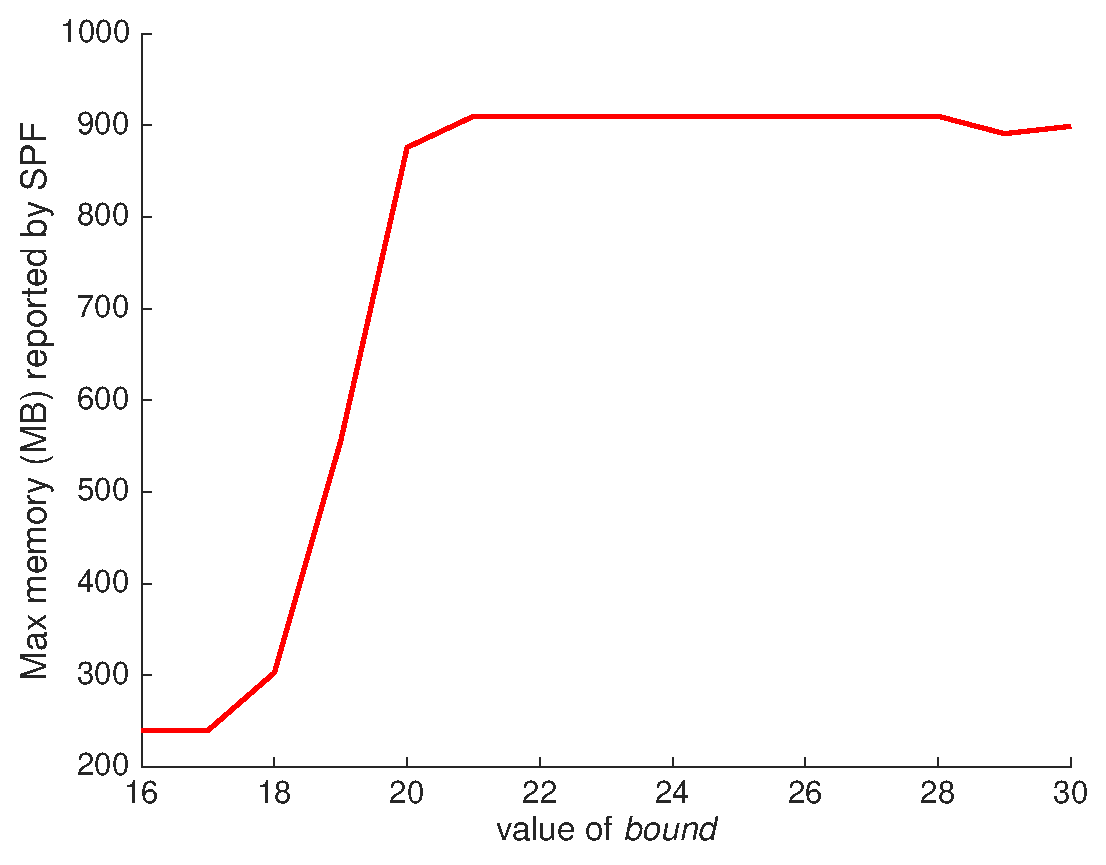
\includegraphics[width=0.4\columnwidth]{figures/sharing_mem} }\label{fig:sharing_mem}}%
    \caption{Time and memory usage of Listing~\ref{lst:sharing} when increasing \textit{bound}}%
    \label{fig:sharing}%
    \vspace{-0.2in}
\end{figure}
%
Figure~\ref{fig:sharing_mem} shows that at a value of 17 for \textit{bound}, the memory usage starts to rise from 240 MB and has reached 910 MB when \textit{bound} equals 21.
%
We also observed that the number of expression objects undergoes a linear increase with the value of \textit{bound}.
%
These three observations lead us to the hypothesis that while SPF does share expression objects internally, the traversal of such expressions breaks the sharing and causes an increase in time and memory.
%
%The time increase is due to garbage collection once the maximum memory threshold is reached.
%
%Integrating veritesting with SPF to make it scale to industrial-sized code requires resolving such engineering issues.
%
\subsection{Complex Expressions}
%Engineering issue \#2: Need to have complex expressions, talk about how Comparators cannot be used anywhere below the top-level operator
During exploration, SPF creates conjunctions of expressions and adds them to its {\em PathCondition} to determine satisfiability of paths.
%
These expressions are allowed to have a \textit{Comparator}~(a comparison operator such as !=) as the top-level operator; however, comparison and Boolean operators are not allowed in sub-expressions.  Thus, the current set of SPF expressions is insufficiently expressive to represent the disjunctive formulas required for multi-path regions.%, and we are currently refactoring the SPF expression hierarchy to allow for richer expression types.
%
%Because SPF has different classes for different expression types~(\textit{IntegerExpressions}, \textit{RealExpression}), these changes must be made in several different places; we believe that moving forward, the
%
%Thus, integrating veritesting presents a design challenge to allow complex expressions in SPF.
%
% \subsection{Intermediate variables}
% %Engineering issue \#3: Nice to introduce intermediate variables
% %
% During veritesting, symbolic formulas derived from static symbolic execution of a region may involve conditional write operations into other variables.
% %
% It is convenient to have intermediate variables~(one per variable written to in the region) which capture such conditional write expressions during the static symbolic execution.
% %
% Later, at an exit point, the intermediate variables can be written into the original variables written to in the region.
% %
% This allows sub-expressions to be shared, and even simplified, without affecting the original variables from the Java bytecode.
% %
% Smaller formulas written into the region\rq s output variables also makes it easier to debug veritesting of regions.
% %
% However, creation of such intermediate variables presents a design challenge in SPF.
% %
% SPF stores and propagates symbolic information through attribute objects.
% %
% This, in turn, creates an invariant that every symbolic variable in the path expression needs to be mapped to an attribute object.

%
%
% \subsection{Veritesting with Multi-threading}
% Veritesting requires SPF to be able to perform static symbolic execution on a region of code and incorporate it as a disjunctive predicate into its path expression along with the corresponding updates to its symbolic store.
% %
% If the region being statically analyzed can be executed in a multi-threaded context, however, then it is necessary to consider all possible points of interference in the region.
% %
% This consideration requires changes to the updates made to SPF\rq s path expression and its symbolic store.
% %
% One way to handle this is to turn every point of interference as an exit point, but determining the possible points of interference statically is itself a difficult problem.  Likely it will require some level of dynamic analysis to determine the points of interference at the time of creation of a veritesting region.
% %
% %But, veritesting would be beneficial if its static analysis also includes computation of points at which interference is infeasible.
% %
% This makes creating an efficient veritesting approach challenging since the cost of this computation must be less than the cost of doing plain dynamic symbolic execution.
















% Data from perl script-based static analysis
% this script just counted the difference between instructions
%
% \begin{table}[]
% \centering
% \caption{My caption}
% \label{my-label}
% \begin{tabular}{|l|l|l|l|}
% \hline
%         & if-ret & if-IV & if-throw \\ \hline
% Chart   & 8.08   & 5.79  & 6.10     \\ \hline
% Closure & 7.40   & 4.37  & 12.6     \\ \hline
% Lang    & 6.3    & 5.23  & 8.26     \\ \hline
% Math    & 12.9   & 6.9   & 9.09     \\ \hline
% Mockito & 8.5    & 4.38  & 11.39    \\ \hline
% Time    & 9.0    & 5.56  & 9.3      \\ \hline
% \end{tabular}
% \end{table}
